
\let\negmedspace\undefined
\let\negthickspace\undefined
\documentclass[journal,12pt,onecolumn]{IEEEtran}
\usepackage{cite}
\usepackage{amsmath,amssymb,amsfonts,amsthm}
\usepackage{algorithmic}
\usepackage{amsmath}
\usepackage{graphicx}
\graphicspath{{./figs/}}
\usepackage{textcomp}
\usepackage{framed} 
\usepackage{lmodern} 
\usepackage{inconsolata}
\usepackage[utf8]{inputenc}
\usepackage{xcolor}
\usepackage{txfonts}
\usepackage{romannum}
\usepackage{listings}
\usepackage{enumitem}
\usepackage{mathtools}
\usepackage{gensymb}
\usepackage{comment}
\usepackage{caption}
\usepackage[breaklinks=true]{hyperref}
\usepackage{tkz-euclide} 
\usepackage{listings}
\usepackage{gvv}                                        
\usepackage{color}        
\usepackage[utf8]{inputenc}                                     
\usepackage{array}                                            
\usepackage{longtable}         
\usepackage{multicol}                              
\usepackage{calc}                                             
\usepackage{multirow}
\usepackage{multicol}
\usepackage{hhline}                                           
\usepackage{ifthen}                                           
\usepackage{lscape}
\usepackage{tabularx}
\usepackage{array}
\usepackage{float}
\newtheorem{theorem}{Theorem}[section]
\newtheorem{problem}{Problem}
\newtheorem{proposition}{Proposition}[section]
\newtheorem{lemma}{Lemma}[section]
\newtheorem{corollary}[theorem]{Corollary}
\newtheorem{example}{Example}[section]
\newtheorem{definition}[problem]{Definition}
\newcommand{\BEQA}{\begin{eqnarray}}
	\newcommand{\EEQA}{\end{eqnarray}}

\theoremstyle{remark}


\title{\textbf{GATE CS 2023}}
\author{ EE25BTECH11052 - Shriyansh Kalpesh Chawda}
\begin{document}
	
	\maketitle
	{\huge GA - General Aptitude}\\
	\\
	\fbox{{\large Q.1 - Q.5 Carry ONE mark each}}\\
	\\
	\begin{enumerate}
		\item We reached the station late, and \underline{\hspace{2cm}} missed the train.
		\hfill{\brak{\text{GATE CS 2023}}}
		
		\begin{enumerate}
			\begin{multicols}{4}
			\item near
			\item nearly
			\item utterly
			\item mostly
						\end{multicols}
		\end{enumerate}
		
		\item Kind $\colon$ \underline{\hspace{2cm}} $\colon$ Often $\colon$ Frequently
		\brak{\text{By word meaning}}
		\hfill{\brak{\text{GATE CS 2023}}}
		
		\begin{enumerate}
			\begin{multicols}{4}
				
			
			\item Mean
			\item Type
			\item Cruel
			\item Kindly
		\end{multicols}
		\end{enumerate}
		
		\item A series of natural numbers $F_1, F_2, F_3, F_4, F_5, F_6, F_7, \dots$ obeys $F_{n+1} = F_n + F_{n-1}$ for all integers $n \geq 2$. If $F_6 = 37$, and $F_7 = 60$, then what is $F_1$ ?
		\hfill{\brak{\text{GATE CS 2023}}}
		
		\begin{enumerate}
			\begin{multicols}{4}
			
			
			\item $4$
			\item $5$
			\item $8$
			\item $9$
		\end{multicols}
		\end{enumerate}
		
		\item A survey for a certain year found that $90\%$ of pregnant women received medical care at least once before giving birth. Of these women, $60\%$ received medical care from doctors, while $40\%$ received medical care from other healthcare providers. Given this information, which one of the following statements can be inferred with \textit{certainty}?
		\hfill{\brak{\text{GATE CS 2023}}}
		
		\begin{enumerate}
			\item More than half of the pregnant women received medical care at least once from a doctor.
			\item Less than half of the pregnant women received medical care at least once from a doctor.
			\item More than half of the pregnant women received medical care at most once from a doctor.
			\item Less than half of the pregnant women received medical care at most once from a doctor.
		\end{enumerate}
		
		\item Looking at the surface of a smooth $3$-dimensional object from the outside, which one of the following options is TRUE?
		\hfill{\brak{\text{GATE CS 2023}}}
		
		\begin{enumerate}
			\item The surface of the object must be concave everywhere.
			\item The surface of the object must be convex everywhere.
			\item The surface of the object may be concave in some places and convex in other places.
			\item The object can have edges, but no corners.
		\end{enumerate}
		
		\item The country of Zombieland is in distress since more than $75\%$ of its working population is suffering from serious health issues. Studies conducted by competent health experts concluded that a complete lack of physical exercise among its working population was one of the leading causes of their health issues. As one of the measures to address the problem, the Government of Zombieland has decided to provide monetary incentives to those who ride bicycles to work.
		
		Based only on the information provided above, which one of the following statements can be logically inferred with \textit{certainty}?
		\hfill{\brak{\text{GATE CS 2023}}}
		
		\begin{enumerate}
			\item All the working population of Zombieland will henceforth ride bicycles to work.
			\item Riding bicycles will ensure that all of the working population of Zombieland is free of health issues.
			\item The health experts suggested to the Government of Zombieland to declare riding bicycles as mandatory.
			\item The Government of Zombieland believes that riding bicycles is a form of physical exercise.
		\end{enumerate}
		
		\item Consider two functions of time \brak{t},
		\begin{align*}
			f\brak{t} &= 0.01 t^2 \\
			g\brak{t} &= 4 t
		\end{align*}
		where $0 < t < \infty$.
		
		Now consider the following two statements:
		\begin{enumerate}
			\item[(i)] For some $t > 0$, $g\brak{t} > f\brak{t}$.
			\item[(ii)] There exists a $T$, such that $f\brak{t} > g\brak{t}$ for all $t > T$.
		\end{enumerate}
		Which one of the following options is TRUE?
		\hfill{\brak{\text{GATE CS 2023}}}
		
		\begin{enumerate}
			\begin{multicols}{2}
			\item only \brak{i} is correct
			\item only \brak{ii} is correct
			\item both \brak{i} and \brak{ii} are correct
			\item neither \brak{i} nor \brak{ii} is correct
		\end{multicols}
		\end{enumerate}
		
		\item Which one of the following sentence sequences creates a coherent narrative?
		\begin{enumerate}

				
			
			\item[(i)] Once on the terrace, on her way to her small room in the corner, she notices the man right away.
			\item[(ii)] She begins to pant by the time she has climbed all the stairs.
			\item[(iii)] Mina has bought vegetables and rice at the market, so her bags are heavy.
			\item[(iv)] He was leaning against the parapet, watching the traffic below.

		\end{enumerate}
			\hfill{\brak{\text{GATE CS 2023}}}
		
		\begin{enumerate}
						\begin{multicols}{2}
			\item \brak{i}, \brak{ii}, \brak{iv}, \brak{iii}
			\item \brak{ii}, \brak{iii}, \brak{i}, \brak{iv}
			\item \brak{iv}, \brak{ii}, \brak{i}, \brak{iii}
			\item \brak{iii}, \brak{ii}, \brak{i}, \brak{iv}
					\end{multicols}
		\end{enumerate}
		
		\item $f\brak{x}$ and $g\brak{y}$ are functions of $x$ and $y$, respectively, and $f\brak{x} = g\brak{y}$ for all real values of $x$ and $y$. Which one of the following options is \textit{necessarily} TRUE for all $x$ and $y$?
		\hfill{\brak{\text{GATE CS 2023}}}
		
		\begin{enumerate}
			\begin{multicols}{2}


			\item $f\brak{x} = 0$ and $g\brak{y} = 0$
			\item $f\brak{x} = g\brak{y} = \text{constant}$
			\item $f\brak{x} \neq \text{constant and } g\brak{y} \neq \text{constant}$
			\item $f\brak{x} + g\brak{y} = f\brak{x} - g\brak{y}$
						\end{multicols}
		\end{enumerate}
		
		\item Which one of the options best describes the transformation of the 2-dimensional figure $P$ to $Q$, and then to $R$, as shown?
\begin{figure}[H]
	\centering
	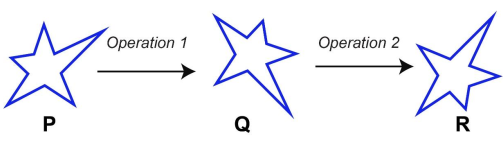
\includegraphics[width=0.3\linewidth]{figs/screenshot001}
	\caption{}
	\label{fig:screenshot001}
\end{figure}
\hfill{\brak{\text{GATE CS 2023}}}
\begin{enumerate}
\item Operation 1: A clockwise rotation by $90\degree$ about an axis perpendicular to the plane of the figure.\\
Operation 2: A reflection along a horizontal line\\
\item Operation 1: A counter clockwise rotation by $90\degree$ about an axis perpendicular to the plane of the figure.\\Operation 2: A reflection along a horizontal line\\
\item Operation 1: A clockwise rotation by $90\degree$ about an axis perpendicular to the plane of the figureOperation 2: A reflection along a vertical line\\
\item Operation 1: A counter clockwise rotation by $180\degree$ about an axis perpendicular to the plane of the figure Operation 2: A reflection along a vertical line\\
\end{enumerate}
			\fbox{{\large Q.11 - Q.35 Carry ONE mark each}}\\
		\item Consider the following statements regarding the front-end and back-end of a compiler.  
		$S1\colon$ The front-end includes phases that are independent of the target hardware.  
		$S2\colon$ The back-end includes phases that are specific to the target hardware.  
		$S3\colon$ The back-end includes phases that are specific to the programming language used in the source code.  
		
		Identify the CORRECT option.
		
\hfill{\brak{\text{GATE CS 2023}}}
		
		\begin{enumerate}
			\begin{multicols}{2}
				\item Only $S1$ is TRUE.
				\item Only $S1$ and $S2$ are TRUE.
				\item $S1$, $S2$, and $S3$ are all TRUE.
				\item Only $S1$ and $S3$ are TRUE.
			\end{multicols}
		\end{enumerate}
		
		\item Which one of the following sequences when stored in an array at locations $A\brak{1}, \ldots, A\brak{10}$ forms a max-heap?
		
\hfill{\brak{\text{GATE CS 2023}}}
		
		\begin{enumerate}
			\begin{multicols}{2}
				\item $23, 17, 10, 6, 13, 14, 1, 5, 7, 12$
				\item $23, 17, 14, 7, 13, 10, 1, 5, 6, 12$
				\item $23, 17, 14, 6, 13, 10, 1, 5, 7, 15$
				\item $23, 14, 17, 1, 10, 13, 16, 12, 7, 5$
			\end{multicols}
		\end{enumerate}
		
		\item Let \texttt{SLLdel} be a function that deletes a node in a singly-linked list given a pointer to the node and a pointer to the head of the list. Similarly, let \texttt{DLLdel} be another function that deletes a node in a doubly-linked list given a pointer to the node and a pointer to the head of the list.  
		
		Let $n$ denote the number of nodes in each of the linked lists. Which one of the following choices is TRUE about the worst-case time complexity of \texttt{SLLdel} and \texttt{DLLdel}?
		
\hfill{\brak{\text{GATE CS 2023}}}
		
		\begin{enumerate}
			\begin{multicols}{2}
				\item \texttt{SLLdel} is $O\brak{1}$ and \texttt{DLLdel} is $O\brak{n}$
				\item Both \texttt{SLLdel} and \texttt{DLLdel} are $O\brak{\log n}$
				\item Both \texttt{SLLdel} and \texttt{DLLdel} are $O\brak{1}$
				\item \texttt{SLLdel} is $O\brak{n}$ and \texttt{DLLdel} is $O\brak{1}$
			\end{multicols}
		\end{enumerate}
		
		\item Consider the Deterministic Finite-state Automaton \brak{DFA} $\mathcal{A}$ shown below. The DFA runs on the alphabet $\brak{0,1}$, and has the set of states $\brak{s, p, q, r}$, with $s$ being the start state and $p$ being the only final state.
		\begin{figure}[H]
			\centering
			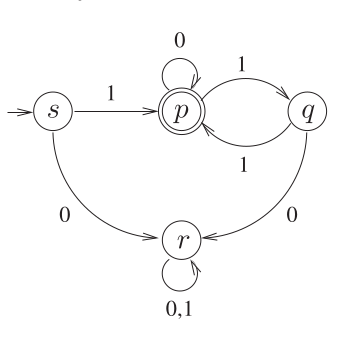
\includegraphics[width=0.3\linewidth]{figs/screenshot020}
			\caption{}
			\label{fig:screenshot020}
		\end{figure}
		
		Which one of the following regular expressions correctly describes the language accepted by $\mathcal{A}$?
		
\hfill{\brak{\text{GATE CS 2023}}}
		
		\begin{enumerate}
			\begin{multicols}{4}
				\item $1\brak{0^{*}11}^{*}$
				\item $0\brak{0+1}^{*}$
				\item $1\brak{0+11}^{*}$
				\item $1\brak{110^{*}}^{*}$
			\end{multicols}
		\end{enumerate}
		
		\item The Lucas sequence $L_n$ is defined by the recurrence relation  
		
		\begin{align*}
			L_n = L_{n-1} + L_{n-2}, \quad \text{for } n \geq 3,
		\end{align*}
		
		with $L_1 = 1$ and $L_2 = 3$.  
		
		Which one of the options given is TRUE?
		
\hfill{\brak{\text{GATE CS 2023}}}
		
		\begin{enumerate}
			\begin{multicols}{2}
				\item $L_n = \brak{\frac{1+\sqrt{5}}{2}}^n + \brak{\frac{1-\sqrt{5}}{2}}^n$
				\item $L_n = \brak{\frac{1+\sqrt{5}}{2}}^n - \brak{\frac{1-\sqrt{5}}{3}}^n$
				\item $L_n = \brak{\frac{1+\sqrt{5}}{2}}^n + \brak{\frac{1-\sqrt{5}}{3}}^n$
				\item $L_n = \brak{\frac{1+\sqrt{5}}{2}}^n - \brak{\frac{1-\sqrt{5}}{2}}^n$
			\end{multicols}
		\end{enumerate}
		
		\item Which one of the options given below refers to the degree \brak{\text{or arity}} of a relation in relational database systems?
		
\hfill{\brak{\text{GATE CS 2023}}}
		
		\begin{enumerate}
			\begin{multicols}{2}
				\item Number of attributes of its relation schema.
				\item Number of tuples stored in the relation.
				\item Number of entries in the relation.
				\item Number of distinct domains of its relation schema.
			\end{multicols}
		\end{enumerate}
		
		\item Suppose two hosts are connected by a point-to-point link and they are configured to use \texttt{Stop-and-Wait} protocol for reliable data transfer. Identify in which one of the following scenarios, the utilization of the link is the lowest.
		
\hfill{\brak{\text{GATE CS 2023}}}
		
		\begin{enumerate}
			\begin{multicols}{2}
				\item Longer link length and lower transmission rate
				\item Longer link length and higher transmission rate
				\item Shorter link length and lower transmission rate
				\item Shorter link length and higher transmission rate
			\end{multicols}
		\end{enumerate}
		
		\item Let 
		$$A = \myvec{1 & 2 & 3 & 4 \\ 4 & 1 & 2 & 3 \\ 3 & 4 & 1 & 2 \\ 2 & 3 & 4 & 1}$$
		
		and 
		
		$$B = \myvec{3 & 4 & 1 & 2 \\ 4 & 1 & 2 & 3 \\ 1 & 2 & 3 & 4 \\ 2 & 3 & 4 & 1}$$
		
		Let $\det\brak{A}$ and $\det\brak{B}$ denote the determinants of the matrices $A$ and $B$, respectively.
		
		Which one of the options given below is TRUE?
		
\hfill{\brak{\text{GATE CS 2023}}}
		
		\begin{enumerate}
			\begin{multicols}{1}
				\item $\det\brak{A} = \det\brak{B}$
				\item $\det\brak{B} = -\det\brak{A}$
				\item $\det\brak{A} = 0$
				\item $\det\brak{AB} = \det\brak{A} + \det\brak{B}$
			\end{multicols}
		\end{enumerate}
		
		\item Consider the following definition of a lexical token id for an identifier in a programming language, using extended regular expressions:
		
		letter $\to$ $[A-Za-z]$
		digit $\to$ $[0-9]$
		id $\to$ letter $\brak{\text{letter } \mid \text{ digit}}^*$
		
		Which one of the following Non-deterministic Finite-state Automata with $\epsilon$-transitions accepts the set of valid identifiers? $\brak{\text{A double-circle denotes a final state}}$
		
\hfill{\brak{\text{GATE CS 2023}}}
		\begin{enumerate}
			\item 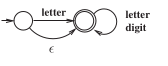
\includegraphics[width=0.3\linewidth]{figs/screenshot005}1
			\item 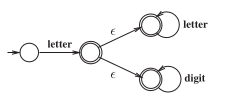
\includegraphics[width=0.3\linewidth]{figs/screenshot006}
			\item 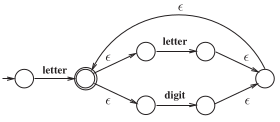
\includegraphics[width=0.3\linewidth]{figs/screenshot007}
			\item 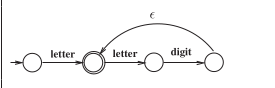
\includegraphics[width=0.4\linewidth]{figs/screenshot008}
			\end{enumerate}
		
		\item An algorithm has to store several keys generated by an adversary in a hash table. The adversary is malicious who tries to maximize the number of collisions. Let $k$ be the number of keys, $m$ be the number of slots in the hash table, and $k > m$.
		
		Which one of the following is the best hashing strategy to counteract the adversary?
		
\hfill{\brak{\text{GATE CS 2023}}}
		
		\begin{enumerate}
	
				\item Division method, i.e., use the hash function $h\brak{k} = k \bmod m$.
				\item Multiplication method, i.e., use the hash function $h\brak{k} = \lfloor m\brak{kA - \lfloor kA \rfloor}\rfloor$, where $A$ is a carefully chosen constant.
				\item Universal hashing method.
				\item If $k$ is a prime number, use Division method. Otherwise, use Multiplication method.

		\end{enumerate}
		
		\item The output of a $2$-input multiplexer is connected back to one of its inputs as shown in the figure.
		\begin{figure}[H]
			\centering
			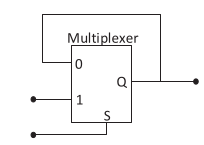
\includegraphics[width=0.3\linewidth]{figs/screenshot002}
			\caption{}
			\label{fig:screenshot002}
		\end{figure}
		
		Match the functional equivalence of this circuit to one of the following options.
		
\hfill{\brak{\text{GATE CS 2023}}}
		
		\begin{enumerate}
			\begin{multicols}{4}
				\item D Flip-flop
				\item D Latch
				\item Half-adder
				\item Demultiplexer
			\end{multicols}
		\end{enumerate}
		
		\item Which one or more of the following need to be saved on a context switch from one thread $\brak{\text{T1}}$ of a process to another thread $\brak{\text{T2}}$ of the same process?
		
\hfill{\brak{\text{GATE CS 2023}}}
		
		\begin{enumerate}
			\begin{multicols}{2}
				\item Page table base register
				\item Stack pointer
				\item Program counter
				\item General purpose registers
			\end{multicols}
		\end{enumerate}
		
		\item Which one or more of the following options guarantee that a computer system will transition from user mode to kernel mode?
		
\hfill{\brak{\text{GATE CS 2023}}}
		
		\begin{enumerate}
			\begin{multicols}{4}
				\item Function Call
				\item malloc Call
				\item Page Fault
				\item System Call
			\end{multicols}
		\end{enumerate}
		
		\item Which of the following statements is/are CORRECT?
		
		\hfill{\brak{\text{GATE CS 2018}}}
		
		\begin{enumerate}
			\begin{multicols}{1}
				\item The intersection of two regular languages is regular.
				\item The intersection of two context-free languages is context-free.
				\item The intersection of two recursive languages is recursive.
				\item The intersection of two recursively enumerable languages is recursively enumerable.
			\end{multicols}
		\end{enumerate}
		
		\item Which of the following statements is/are INCORRECT about the OSPF $\brak{\text{Open Shortest Path First}}$ routing protocol used in the Internet?
		
\hfill{\brak{\text{GATE CS 2023}}}
		
		\begin{enumerate}
			\begin{multicols}{1}
				\item OSPF implements Bellman-Ford algorithm to find shortest paths.
				\item OSPF uses Dijkstra's shortest path algorithm to implement least-cost path routing.
				\item OSPF is used as an inter-domain routing protocol.
				\item OSPF implements hierarchical routing.
			\end{multicols}
		\end{enumerate}
		
		\item Geetha has a conjecture about integers, which is of the form
		$$\forall x \brak{P\brak{x} \Rightarrow \exists yQ\brak{x,y}},$$
		
		where $P$ is a statement about integers, and $Q$ is a statement about pairs of integers. Which of the following $\brak{\text{one or more}}$ option$\brak{s}$ would imply Geetha's conjecture?
		
\hfill{\brak{\text{GATE CS 2023}}}
		
		\begin{enumerate}
			\begin{multicols}{1}
				\item $\exists x \brak{P\brak{x} \land \forall yQ\brak{x,y}}$
				\item $\forall x\forall yQ\brak{x,y}$
				\item $\exists y\forall x \brak{P\brak{x} \Rightarrow Q\brak{x,y}}$
				\item $\exists x \brak{P\brak{x} \land \exists yQ\brak{x,y}}$
			\end{multicols}
		\end{enumerate}
		\item Which one or more of the following CPU scheduling algorithms can potentially cause starvation?
		
		\hfill{\brak{\text{GATE CS 2023}}}
		
		\begin{enumerate}
			\begin{multicols}{2}
				\item First-in First-Out
				\item Round Robin
				\item Priority Scheduling
				\item Shortest Job First
			\end{multicols}
		\end{enumerate}
		
		\item Let 
		$$f\brak{x} = x^3 + 15x^2 - 33x - 36$$
		be a real-valued function.
		
		Which of the following statements is/are TRUE?
		
		\hfill{\brak{\text{GATE CS 2023}}}
		
		\begin{enumerate}
			\begin{multicols}{1}
				\item $f\brak{x}$ does not have a local maximum.
				\item $f\brak{x}$ has a local maximum.
				\item $f\brak{x}$ does not have a local minimum.
				\item $f\brak{x}$ has a local minimum.
			\end{multicols}
		\end{enumerate}
		
		\item Let $f$ and $g$ be functions of natural numbers given by $f\brak{n} = n$ and $g\brak{n} = n^2$. Which of the following statements is/are TRUE?
		
		\hfill{\brak{\text{GATE CS 2023}}}
		
		\begin{enumerate}
			\begin{multicols}{4}
				\item $f \in O\brak{g}$
				\item $f \in \Omega\brak{g}$
				\item $f \in o\brak{g}$
				\item $f \in \Theta\brak{g}$
			\end{multicols}
		\end{enumerate}
		
		\item Let $A$ be the adjacency matrix of the graph with vertices $\{1, 2, 3, 4, 5\}$.
\begin{figure}[H]
	\centering
	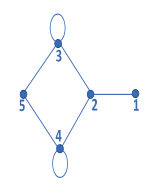
\includegraphics[width=0.3\linewidth]{figs/screenshot009}
	\caption{}
	\label{fig:screenshot009}
\end{figure}
		
		Let $\lambda_1, \lambda_2, \lambda_3, \lambda_4$, and $\lambda_5$ be the five eigenvalues of $A$. Note that these eigenvalues need not be distinct.
		The value of $\lambda_1 + \lambda_2 + \lambda_3 + \lambda_4 + \lambda_5 = $ \underline{\hspace{2cm}}
		
		\hfill{\brak{\text{GATE CS 2023}}}
		
		\item The value of the definite integral
		$$\int_{-3}^{3} \int_{-2}^{2} \int_{-1}^{1} \brak{4x^2 y - z^3} \, dz \, dy \, dx$$
		
		is \underline{\hspace{2cm}}. $\brak{\text{Rounded off to the nearest integer}}$
		
		\hfill{\brak{\text{GATE CS 2023}}}
		
		\item A particular number is written as $132$ in radix-$4$ representation. The same number in radix-$5$ representation is \underline{\hspace{2cm}}
		
		\hfill{\brak{\text{GATE CS 2023}}}
		
		\item Consider a $3$-stage pipelined processor having a delay of $10$ ns $\brak{\text{nanoseconds}}$, $20$ ns, and $14$ ns, for the first, second, and the third stages, respectively. Assume that there is no other delay and the processor does not suffer from any pipeline hazards. Also assume that one instruction is fetched every cycle.
		The total execution time for executing $100$ instructions on this processor is \underline{\hspace{2cm}} ns.
		
		\hfill{\brak{\text{GATE CS 2023}}}
		
		\item A keyboard connected to a computer is used at a rate of $1$ keystroke per second. The computer system polls the keyboard every $10$ ms $\brak{\text{milli seconds}}$ to check for a keystroke and consumes $100$ $\mu$ $\brak{\text{micro seconds}}$ for each poll. If it is determined after polling that a key has been pressed, the system consumes an additional $200$ $\mu$s to process the keystroke. Let $T_1$ denote the fraction of a second spent in polling and processing a keystroke.
		
		In an alternative implementation, the system uses interrupts instead of polling. An interrupt is raised for every keystroke. It takes a total of $1$ ms for servicing an interrupt and processing a keystroke. Let $T_2$ denote the fraction of a second spent in servicing the interrupt and processing a keystroke.
		
		The ratio $\frac{T_1}{T_2}$ is \underline{\hspace{2cm}}. $\brak{\text{Rounded off to one decimal place}}$
		
		\hfill{\brak{\text{GATE CS 2023}}}
		
		\item The integer value printed by the ANSI-C program given below is \underline{\hspace{2cm}}.
		
		\begin{verbatim}
			#include<stdio.h>
			int funcp(){
				static int x = 1;
				x++;
				return x;
			}
			int main(){
				int x,y;
				x = funcp();
				y = funcp()+x;
				printf("%d\n", (x+y));
				return 0;
			}
		\end{verbatim}
		
		\hfill{\brak{\text{GATE CS 2023}}}\\
		\fbox{{\large Q.36 - Q.65 Carry ONE mark each}}\\
		\item Consider the following program:
		
		\begin{verbatim}
			int main()
			{
				f1();
				f2(2);
				f3();
				return(0);
			}
					\end{verbatim}
					\underline{\hspace{9cm}}
					\begin{verbatim}
			int f1()
			{
				return(1);
			}
					\end{verbatim}
					\underline{\hspace{9cm}}
							\begin{verbatim}
			int f2(int X)
			{
				f3();
				if (X==1)
				return f1();
				else
				return (X*f2(X-1));
			}
					\end{verbatim}
					\underline{\hspace{9cm}}
							\begin{verbatim}
			int f3()
			{
				return(5);
			}
		\end{verbatim}
		
		Which one of the following options represents the activation tree corresponding to the main function?
		
		\hfill{\brak{\text{GATE CS 2023}}}
		\begin{enumerate}
						\begin{multicols}{2}
				\item
				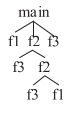
\includegraphics[width=0.3\linewidth]{figs/screenshot010}
				\item 
				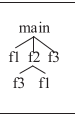
\includegraphics[width=0.3\linewidth]{figs/screenshot011}
				\item 
				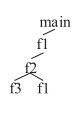
\includegraphics[width=0.3\linewidth]{figs/screenshot012}
				\item
				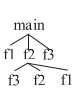
\includegraphics[width=0.3\linewidth]{figs/screenshot013}
				
			\end{multicols}
		\end{enumerate}
\item Consider the control flow graph shown.
\begin{figure}[H]
	\centering
	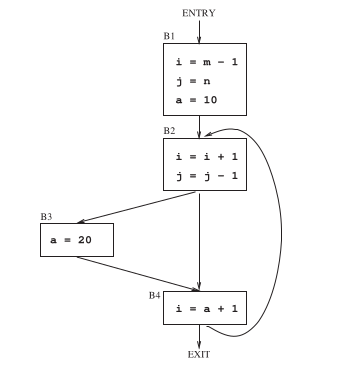
\includegraphics[width=0.5\linewidth]{figs/screenshot003}
	\caption{}
	\label{fig:screenshot003}
\end{figure}


		
		Which one of the following choices correctly lists the set of live variables at the exit point of each basic block?
		
		\hfill{\brak{\text{GATE CS 2023}}}
		
		\begin{enumerate}
			\begin{multicols}{1}
				\item $B1\colon \{\}$, $B2\colon \{a\}$, $B3\colon \{a\}$, $B4\colon \{a\}$
				\item $B1\colon \{i, j\}$, $B2\colon \{a\}$, $B3\colon \{a\}$, $B4\colon \{i\}$
				\item $B1\colon \{a, i, j\}$, $B2\colon \{a, i, j\}$, $B3\colon \{a, i\}$, $B4\colon \{a\}$
				\item $B1\colon \{a, i, j\}$, $B2\colon \{a, j\}$, $B3\colon \{a, j\}$, $B4\colon \{a, i, j\}$
			\end{multicols}
		\end{enumerate}
		
	\item Consider the two functions incr and decr shown below.
	
	\begin{minipage}{0.45\textwidth}
		\begin{verbatim}
			incr(){
				wait(s);
				X = X+1;
				signal(s);
			}
		\end{verbatim}
	\end{minipage}
	\hfill
	\vrule
	\hfill
	\begin{minipage}{0.45\textwidth}
		\begin{verbatim}
			decr(){
				wait(s);
				X = X-1;
				signal(s);
			}
		\end{verbatim}
	\end{minipage}
	
	There are $5$ threads each invoking incr once, and $3$ threads each invoking decr once, on the same shared variable $X$. The initial value of $X$ is $10$.
	
	Suppose there are two implementations of the semaphore $s$, as follows: I-$1$: $s$ is a binary semaphore initialized to $1$. I-$2$: $s$ is a counting semaphore initialized to $2$.
	
	Let $V_1$, $V_2$ be the values of $X$ at the end of execution of all the threads with implementations I-$1$, I-$2$, respectively.
	
	Which one of the following choices corresponds to the minimum possible values of $V_1$, $V_2$, respectively?
	
	\hfill $\brak{\text{GATE CS 2023}}$
	
	\begin{enumerate}
		\begin{multicols}{4}
			\item $15$, $7$
			\item $7$, $7$
			\item $12$, $7$
			\item $12$, $8$
		\end{multicols}
	\end{enumerate}

		
		\item Consider the context-free grammar $G$ below
		$$S \to aSb \mid X$$
		$$X \to aX \mid Xb \mid a \mid b,$$
		where $S$ and $X$ are non-terminals, and $a$ and $b$ are terminal symbols. The starting non-terminal is $S$.
		
		Which one of the following statements is CORRECT?
		
		\hfill{\brak{\text{GATE CS 2023}}}
		
		\begin{enumerate}

				\item The language generated by $G$ is $\brak{a + b}^*$
				\item The language generated by $G$ is $a^* \brak{a + b} b^*$
				\item The language generated by $G$ is $a^* b^* \brak{a + b}$
				\item The language generated by $G$ is not a regular language

		\end{enumerate}
		
		\item Consider the pushdown automaton $\brak{\text{PDA}}$ $P$ below, which runs on the input alphabet $\{a, b\}$, has stack alphabet $\{\perp, A\}$, and has three states $\{s, p, q\}$, with $s$ being the start state. A transition from state $u$ to state $v$, labelled $c/X/\gamma$, where $c$ is an input symbol or $\epsilon$, $X$ is a stack symbol, and $\gamma$ is a string of stack symbols, represents the fact that in state $u$, the PDA can read $c$ from the input, with $X$ on the top of its stack, pop $X$ from the stack, push in the string $\gamma$ on the stack, and go to state $v$. In the initial configuration, the stack has only the symbol $\perp$ in it. The PDA accepts by empty stack.
\begin{figure}[H]
	\centering
	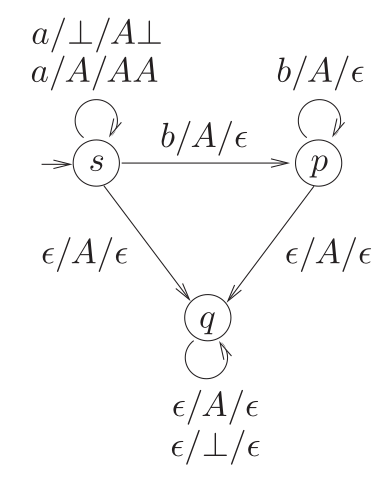
\includegraphics[width=0.3\linewidth]{figs/screenshot014}
	\caption{}
	\label{fig:screenshot014}
\end{figure}
		
		Which one of the following options correctly describes the language accepted by $P$?
		
		\hfill{\brak{\text{GATE CS 2023}}}
		
		\begin{enumerate}
			\begin{multicols}{1}
				\item $\{a^m b^n \mid 1 \leq m \text{ and } n < m\}$
				\item $\{a^m b^n \mid 0 \leq n \leq m\}$
				\item $\{a^m b^n \mid 0 \leq m \text{ and } 0 \leq n\}$
				\item $\{a^m \mid 0 \leq m\} \cup \{b^n \mid 0 \leq n\}$
			\end{multicols}
		\end{enumerate}
		
		\item Consider the given C-code and its corresponding assembly code, with a few operands $U1$–$U4$ being unknown. Some useful information as well as the semantics of each unique assembly instruction is annotated as inline comments in the code. The memory is byte-addressable.
		
		\begin{verbatim}
			//C-code
			int a[10], b[10], i;
			// int is 32-bit
			for (i=0; i<10;i++)
			a[i] = b[i] * 8;
		\end{verbatim}
		\underline{\hspace{9cm}}
		\begin{verbatim}
			;assembly-code (; indicates comments)
			;r1-r5 are 32-bit integer registers
			;initialize r1=0, r2=10
			;initialize r3, r4 with base address of a, b
			L01: jeq r1, r2, end ;if(r1==r2) goto end
			L02: lw r5, 0(r4) ;r5 <- Memory[r4+0]
			L03: shl r5, r5, U1 ;r5 <- r5 << U1
			L04: sw r5, 0(r3) ;Memory[r3+0] <- r5
			L05: add r3, r3, U2 ;r3 <- r3+U2
			L06: add r4, r4, U3
			L07: add r1, r1, 1
			L08: jmp U4 ;goto U4
			L09: end
		\end{verbatim}
		
		Which one of the following options is a CORRECT replacement for operands in the position $\brak{U1, U2, U3, U4}$ in the above assembly code?
		
		\hfill{\brak{\text{GATE CS 2023}}}
		
		\begin{enumerate}
			\begin{multicols}{2}
				\item $\brak{8, 4, 1, L02}$
				\item $\brak{3, 4, 4, L01}$
				\item $\brak{8, 1, 1, L02}$
				\item $\brak{3, 1, 1, L01}$
			\end{multicols}
		\end{enumerate}
		
		\item A $4$ kilobyte $\brak{\text{KB}}$ byte-addressable memory is realized using four $1$ KB memory blocks. Two input address lines $\brak{IA4 \text{ and } IA3}$ are connected to the chip select $\brak{\text{CS}}$ port of these memory blocks through a decoder as shown in the figure. The remaining ten input address lines from $IA11$–$IA0$ are connected to the address port of these blocks. The chip select $\brak{\text{CS}}$ is active high.
\begin{figure}[H]
	\centering
	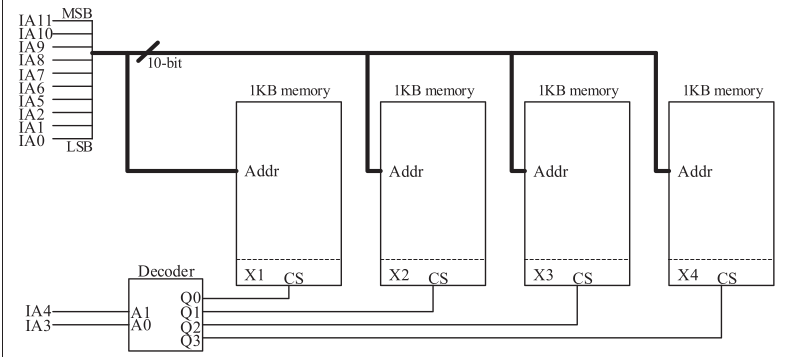
\includegraphics[width=0.5\linewidth]{figs/screenshot015}
	\caption{}
	\label{fig:screenshot015}
\end{figure}
		
		

		
		The input memory addresses $\brak{IA11–IA0}$, in decimal, for the starting locations $\brak{Addr=0}$ of each block $\brak{\text{indicated as } X1, X2, X3, X4 \text{ in the figure}}$ are among the options given below. Which one of the following options is CORRECT?
		
		\hfill{\brak{\text{GATE CS 2023}}}
		
		\begin{enumerate}
			\begin{multicols}{2}
				\item $\brak{0, 1, 2, 3}$
				\item $\brak{0, 1024, 2048, 3072}$
				\item $\brak{0, 8, 16, 24}$
				\item $\brak{0, 0, 0, 0}$
			\end{multicols}
		\end{enumerate}
		
		\item Consider a sequential digital circuit consisting of T flip-flops and D flip-flops as shown in the figure. CLKIN is the clock input to the circuit. At the beginning, $Q1, Q2$ and $Q3$ have values $0, 1$ and $1$, respectively.
		\begin{figure}[H]
			\centering
			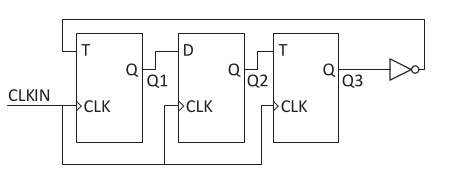
\includegraphics[width=0.5\linewidth]{figs/screenshot016}
			\caption{}
			\label{fig:screenshot016}
		\end{figure}
		

		
		Which one of the given values of $\brak{Q1, Q2, Q3}$ can NEVER be obtained with this digital circuit?
		
		\hfill{\brak{\text{GATE CS 2023}}}
		
		\begin{enumerate}
			\begin{multicols}{4}
				\item $\brak{0, 0, 1}$
				\item $\brak{1, 0, 0}$
				\item $\brak{1, 0, 1}$
				\item $\brak{1, 1, 1}$
			\end{multicols}
		\end{enumerate}
		
		\item A Boolean digital circuit is composed using two $4$-input multiplexers $\brak{M1 \text{ and } M2}$ and one $2$-input multiplexer $\brak{M3}$ as shown in the figure. $X0$–$X7$ are the inputs of the multiplexers $M1$ and $M2$ and could be connected to either $0$ or $1$. The select lines of the multiplexers are connected to Boolean variables $A, B$ and $C$ as shown.
		\begin{figure}[H]
			\centering
			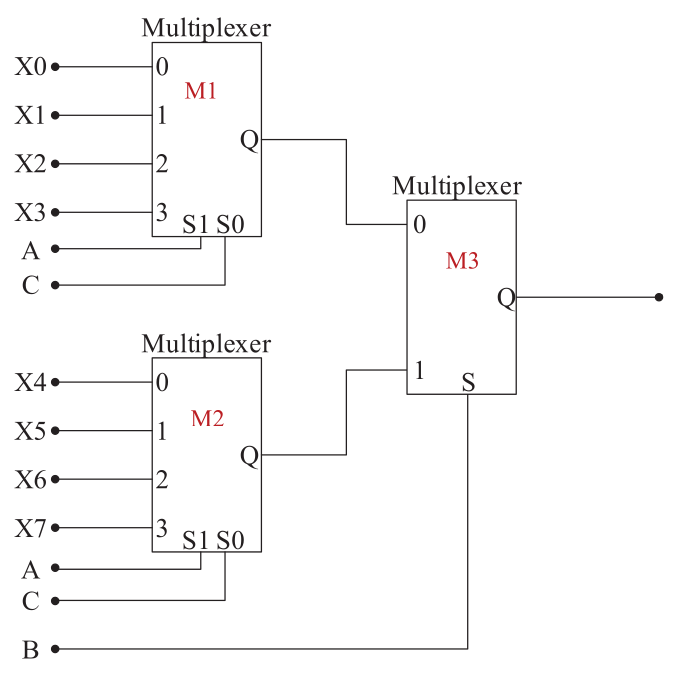
\includegraphics[width=0.5\linewidth]{figs/screenshot017}
			\caption{}
			\label{fig:screenshot017}
		\end{figure}
		

		
		Which one of the following set of values of $\brak{X0, X1, X2, X3, X4, X5, X6, X7}$ will realise the Boolean function $A + \overline{A}.C + A.\overline{
		B}.C$?
		
		\hfill{\brak{\text{GATE CS 2023}}}
		
		\begin{enumerate}
			\begin{multicols}{1}
				\item $\brak{1, 1, 0, 0, 1, 1, 1, 0}$
				\item $\brak{1, 1, 0, 0, 1, 1, 0, 1}$
				\item $\brak{1, 1, 0, 1, 1, 1, 0, 0}$
				\item $\brak{0, 0, 1, 1, 0, 1, 1, 1}$
			\end{multicols}
		\end{enumerate}
		
		\item Consider the IEEE-754 single precision floating point numbers
		$P=0xC1800000$ and $Q=0x3F5C2EF4$.
		Which one of the following corresponds to the product of these numbers $\brak{\text{i.e., } P \times Q}$, represented in the IEEE-754 single precision format?
		
		\hfill{\brak{\text{GATE CS 2023}}}
		
		\begin{enumerate}
			\begin{multicols}{4}
				\item $0x404C2EF4$
				\item $0x405C2EF4$
				\item $0xC15C2EF4$
				\item $0xC14C2EF4$
			\end{multicols}
		\end{enumerate}
		
		\item Let $A$ be a priority queue for maintaining a set of elements. Suppose $A$ is implemented using a max-heap data structure. The operation Extract-Max$\brak{A}$ extracts and deletes the maximum element from $A$. The operation Insert$\brak{A,\text{key}}$ inserts a new element key in $A$. The properties of a max-heap are preserved at the end of each of these operations.
		
		When $A$ contains $n$ elements, which one of the following statements about the worst case running time of these two operations is TRUE?
		
		\hfill{\brak{\text{GATE CS 2023}}}
		
		\begin{enumerate}
			\begin{multicols}{1}
				\item Both Extract-Max$\brak{A}$ and Insert$\brak{A,\text{key}}$ run in $O\brak{1}$.
				\item Both Extract-Max$\brak{A}$ and Insert$\brak{A,\text{key}}$ run in $O\brak{\log\brak{n}}$.
				\item Extract-Max$\brak{A}$ runs in $O\brak{1}$ whereas Insert$\brak{A,\text{key}}$ runs in $O\brak{n}$.
				\item Extract-Max$\brak{A}$ runs in $O\brak{1}$ whereas Insert$\brak{A,\text{key}}$ runs in $O\brak{\log\brak{n}}$.
			\end{multicols}
		\end{enumerate}
		
		\item Consider the C function foo and the binary tree shown.
		
		\begin{verbatim}
			typedef struct node {
				int val;
				struct node *left, *right;
			} node;
			
			int foo(node *p) {
				int retval;
				if (p == NULL)
				return 0;
				else {
					retval = p->val + foo(p->left) + foo(p->right);
					printf("%d ", retval);
					return retval;
				}
			}
		\end{verbatim}
	\begin{figure}[H]
			\centering
			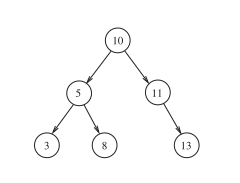
\includegraphics[width=0.3\linewidth]{figs/screenshot018}
			\caption{}
			\label{fig:screenshot018}
		\end{figure}
		
		

		
		When foo is called with a pointer to the root node of the given binary tree, what will it print?
		
		\hfill{\brak{\text{GATE CS 2023}}}
		
		\begin{enumerate}
			\begin{multicols}{2}
				\item $3$ $8$ $5$ $13$ $11$ $10$
				\item $3$ $5$ $8$ $10$ $11$ $13$
				\item $3$ $8$ $16$ $13$ $24$ $50$
				\item $3$ $16$ $8$ $50$ $24$ $13$
			\end{multicols}
		\end{enumerate}
		
		\item Let $U = \{1, 2, \ldots, n\}$, where $n$ is a large positive integer greater than $1000$. Let $k$ be a positive integer less than $n$. Let $A, B$ be subsets of $U$ with $|A| = |B| = k$ and $A \cap B = \emptyset$. We say that a permutation of $U$ separates $A$ from $B$ if one of the following is true.
		\begin{itemize}
			\item All members of $A$ appear in the permutation before any of the members of $B$.
			\item All members of $B$ appear in the permutation before any of the members of $A$.
		\end{itemize}
		How many permutations of $U$ separate $A$ from $B$?
		
		\hfill{\brak{\text{GATE CS 2023}}}
		
		\begin{enumerate}
			\begin{multicols}{1}
				\item $n!$
				\item $\binom{n}{2k} \brak{n - 2k}!$
				\item $\binom{n}{2k} \brak{n - 2k}! \brak{k!}^2$
				\item $2 \binom{n}{2k} \brak{n - 2k}! \brak{k!}^2$
			\end{multicols}
		\end{enumerate}
		
		\item Let $f \colon A \to B$ be an onto $\brak{\text{or surjective}}$ function, where $A$ and $B$ are nonempty sets. Define an equivalence relation $\sim$ on the set $A$ as
		$$a_1 \sim a_2 \text{ if } f\brak{a_1} = f\brak{a_2},$$
		where $a_1, a_2 \in A$. Let $E = \{[x] \colon x \in A\}$ be the set of all the equivalence classes under $\sim$. Define a new mapping $F \colon E \to B$ as
		$$F\brak{[x]} = f\brak{x}, \text{ for all the equivalence classes } [x] \text{ in } E.$$
		
		Which of the following statements is/are TRUE?
		
		\hfill{\brak{\text{GATE CS 2023}}}
		
		\begin{enumerate}
			\begin{multicols}{1}
				\item $F$ is NOT well-defined.
				\item $F$ is an onto $\brak{\text{or surjective}}$ function.
				\item $F$ is a one-to-one $\brak{\text{or injective}}$ function.
				\item $F$ is a bijective function.
			\end{multicols}
		\end{enumerate}
		
		\item Suppose you are asked to design a new reliable byte-stream transport protocol like TCP. This protocol, named myTCP, runs over a $100$ Mbps network with Round Trip Time of $150$ milliseconds and the maximum segment lifetime of $2$ minutes. Which of the following is/are valid lengths of the Sequence Number field in the myTCP header?
		
		\hfill{\brak{\text{GATE CS 2023}}}
		
		\begin{enumerate}
			\begin{multicols}{4}
				\item $30$ bits
				\item $32$ bits
				\item $34$ bits
				\item $36$ bits
			\end{multicols}
		\end{enumerate}
		
		\item Let $X$ be a set and $2^X$ denote the powerset of $X$.
		Define a binary operation $\Delta$ on $2^X$ as follows:
		$$A\Delta B = \brak{A - B} \cup \brak{B - A}.$$
		Let $H = \brak{2^X, \Delta}$. Which of the following statements about $H$ is/are correct?
		
		\hfill{\brak{\text{GATE CS 2023}}}
		
		\begin{enumerate}
			\begin{multicols}{1}
				\item $H$ is a group.
				\item Every element in $H$ has an inverse, but $H$ is NOT a group.
				\item For every $A \in 2^X$, the inverse of $A$ is the complement of $A$.
				\item For every $A \in 2^X$, the inverse of $A$ is $A$.
			\end{multicols}
		\end{enumerate}
		
		\item Suppose in a web browser, you click on the www.gate-2023.in URL. The browser cache is empty. The IP address for this URL is not cached in your local host, so a DNS lookup is triggered $\brak{\text{by the local DNS server deployed on your local host}}$ over the $3$-tier DNS hierarchy in an iterative mode. No resource records are cached anywhere across all DNS servers.
		
		Let RTT denote the round trip time between your local host and DNS servers in the DNS hierarchy. The round trip time between the local host and the web server hosting www.gate-2023.in is also equal to RTT. The HTML file associated with the URL is small enough to have negligible transmission time and negligible rendering time by your web browser, which references $10$ equally small objects on the same web server.
		
		Which of the following statements is/are CORRECT about the minimum elapsed time between clicking on the URL and your browser fully rendering it?
		
		\hfill{\brak{\text{GATE CS 2023}}}
		
		\begin{enumerate}
				\item $7$ RTTs, in case of non-persistent HTTP with $5$ parallel TCP connections.
				\item $5$ RTTs, in case of persistent HTTP with pipelining.
				\item $9$ RTTs, in case of non-persistent HTTP with $5$ parallel TCP connections.
				\item $6$ RTTs, in case of persistent HTTP with pipelining.
		\end{enumerate}
		
		\item Consider a random experiment where two fair coins are tossed. Let $A$ be the event that denotes HEAD on both the throws, $B$ be the event that denotes HEAD on the first throw, and $C$ be the event that denotes HEAD on the second throw.
		
		Which of the following statements is/are TRUE?
		
		\hfill{\brak{\text{GATE CS 2023}}}
		
		\begin{enumerate}
			\begin{multicols}{2}
				\item $A$ and $B$ are independent.
				\item $A$ and $C$ are independent.
				\item $B$ and $C$ are independent.
				\item Prob$\brak{B|C} =$ Prob$\brak{B}$
			\end{multicols}
		\end{enumerate}
		
		\item Consider functions Function $1$ and Function $2$ expressed in pseudocode as follows:
		
		\begin{minipage}{0.45\textwidth}
			\textbf{Function 1}
			\begin{verbatim}
				while n > 1 do
				for i = 1 to n do
				x = x + 1;
				end for
				n = n/2;
				end while
			\end{verbatim}
		\end{minipage}
		\hfill
		\vrule
		\hfill
		\begin{minipage}{0.45\textwidth}
			\textbf{Function 2}
			\begin{verbatim}
				for i = 1 to 100 * n do
				x = x + 1;
				end for
			\end{verbatim}
		\end{minipage}
		
		Let $f_1\brak{n}$ and $f_2\brak{n}$ denote the number of times the statement "$x = x + 1$" is executed in Function $1$ and Function $2$, respectively.
		
		Which of the following statements is/are TRUE?
		
		\hfill $\brak{\text{GATE CS 2023}}$
		
		\begin{enumerate}
			\begin{multicols}{2}
				\item $f_1\brak{n} \in \Theta\brak{f_2\brak{n}}$
				\item $f_1\brak{n} \in o\brak{f_2\brak{n}}$
				\item $f_1\brak{n} \in \omega\brak{f_2\brak{n}}$
				\item $f_1\brak{n} \in O\brak{n}$
			\end{multicols}
		\end{enumerate}
		
	
		
		\item Let $G$ be a simple, finite, undirected graph with vertex set $\{v_1, \ldots, v_n\}$. Let $\Delta\brak{G}$ denote the maximum degree of $G$ and let $N = \{1, 2, \ldots\}$ denote the set of all possible colors. Color the vertices of $G$ using the following greedy strategy:
		\begin{verbatim}
			for i = 1, \dots, n
			color(v_i) <- min{j in N : no neighbour of v_i is colored j}
		\end{verbatim}
		
		Which of the following statements is/are TRUE?
		
		\hfill{\brak{\text{GATE CS 2023}}}
		
		\begin{enumerate}

				\item This procedure results in a proper vertex coloring of $G$.
				\item The number of colors used is at most $\Delta\brak{G} + 1$.
				\item The number of colors used is at most $\Delta\brak{G}$.
				\item The number of colors used is equal to the chromatic number of $G$.

		\end{enumerate}
		
		\item Let $U = \{1, 2, 3\}$. Let $2^U$ denote the powerset of $U$. Consider an undirected graph $G$ whose vertex set is $2^U$. For any $A, B \in 2^U$, $\brak{A, B}$ is an edge in $G$ if and only if $\brak{i}$ $A \neq B$, and $\brak{ii}$ either $A \subseteq B$ or $B \subseteq A$. For any vertex $A$ in $G$, the set of all possible orderings in which the vertices of $G$ can be visited in a Breadth First Search $\brak{\text{BFS}}$ starting from $A$ is denoted by $B\brak{A}$.
		
		If $\emptyset$ denotes the empty set, then the cardinality of $B\brak{\emptyset}$ is \underline{\hspace{2cm}}.
		
		\hfill{\brak{\text{GATE CS 2023}}}
		
		\item Consider the following two-dimensional array $D$ in the C programming language, which is stored in row-major order:
		\begin{verbatim}
			int D[128][128];
		\end{verbatim}
		
		Demand paging is used for allocating memory and each physical page frame holds $512$ elements of the array $D$. The Least Recently Used $\brak{\text{LRU}}$ page-replacement policy is used by the operating system. A total of $30$ physical page frames are allocated to a process which executes the following code snippet:
		
		\begin{verbatim}
			for (int i = 0; i < 128; i++)
			for (int j = 0; j < 128; j++)
			D[j][i] *= 10;
		\end{verbatim}
		
		The number of page faults generated during the execution of this code snippet is \underline{\hspace{2cm}}.
		
		\hfill{\brak{\text{GATE CS 2023}}}
			
			\item Consider a computer system with $57$-bit virtual addressing using multi-level tree-structured page tables with $L$ levels for virtual to physical address translation. The page size is $4$ KB $\brak{1 \text{ KB} = 1024 \text{ B}}$ and a page table entry at any of the levels occupies $8$ bytes.
			
			The value of $L$ is \underline{\hspace{2cm}}.
			
			\hfill $\brak{\text{GATE CS 2023}}$
			
			\item Consider a sequence $a$ of elements $a_0 = 1$, $a_1 = 5$, $a_2 = 7$, $a_3 = 8$, $a_4 = 9$, and $a_5 = 2$. The following operations are performed on a stack $S$ and a queue $Q$, both of which are initially empty.
			
			I: push the elements of $a$ from $a_0$ to $a_5$ in that order into $S$.
			
			II: enqueue the elements of $a$ from $a_0$ to $a_5$ in that order into $Q$.
			
			III: pop an element from $S$.
			
			IV: dequeue an element from $Q$.
			
			V: pop an element from $S$.
			
			VI: dequeue an element from $Q$.
			
			VII: dequeue an element from $Q$ and push the same element into $S$.
			
			VIII: Repeat operation VII three times.
			
			IX: pop an element from $S$.
			
			X: pop an element from $S$.
			
			The top element of $S$ after executing the above operations is \underline{\hspace{2cm}}.
			
			\hfill $\brak{\text{GATE CS 2023}}$
			
			\item Consider the syntax directed translation given by the following grammar and semantic rules. Here $N$, $I$, $F$ and $B$ are non-terminals. $N$ is the starting non-terminal, and $\#$, $0$ and $1$ are lexical tokens corresponding to input letters "$\#$", "$0$" and "$1$", respectively. $X.\text{val}$ denotes the synthesized attribute $\brak{\text{a numeric value}}$ associated with a non-terminal $X$. $I_1$ and $F_1$ denote occurrences of $I$ and $F$ on the right hand side of a production, respectively. For the tokens $0$ and $1$, $0.\text{val} = 0$ and $1.\text{val} = 1$.
			
			\begin{align*}
				N &\to I \# F &&N.\text{val} = I.\text{val} + F.\text{val}\\
				I &\to I_1 B &&I.\text{val} = \brak{2 \cdot I_1.\text{val}} + B.\text{val}\\
				I &\to B &&I.\text{val} = B.\text{val}\\
				F &\to B F_1 &&F.\text{val} = \frac{1}{2}\brak{B.\text{val} + F_1.\text{val}}\\
				F &\to B &&F.\text{val} = \frac{1}{2}B.\text{val}\\
				B &\to 0 &&B.\text{val} = 0.\text{val}\\
				B &\to 1 &&B.\text{val} = 1.\text{val}
			\end{align*}
			
			The value computed by the translation scheme for the input string $10\#011$ is \underline{\hspace{2cm}}.\\
			 $\brak{\text{Rounded off to three decimal places}}$
			
			\hfill $\brak{\text{GATE CS 2023}}$
			
			\item Consider the following table named Student in a relational database. The primary key of this table is rollNum.
			
			\begin{table}[h]
				\centering
				\caption*{}
				\label{tab:student}
				\begin{tabular}{|c|c|c|c|}
					\hline
					rollNum & name & gender & marks \\
					\hline
					$1$ & Naman & M & $62$ \\
					\hline
					$2$ & Aliya & F & $70$ \\
					\hline
					$3$ & Aliya & F & $80$ \\
					\hline
					$4$ & James & M & $82$ \\
					\hline
					$5$ & Swati & F & $65$ \\
					\hline
				\end{tabular}
			\end{table}
The SQL query below is executed on this database.	
			\begin{verbatim}
				SELECT *
				FROM Student
				WHERE gender = 'F' AND
				marks > 65;
				
			\end{verbatim}
			
			The number of rows returned by the query is \underline{\hspace{2cm}}.
			
			\hfill $\brak{\text{GATE CS 2023}}$
			
			\item Consider a database of fixed-length records, stored as an ordered file. The database has $25{,}000$ records, with each record being $100$ bytes, of which the primary key occupies $15$ bytes. The data file is block-aligned in that each data record is fully contained within a block. The database is indexed by a primary index file, which is also stored as a block-aligned ordered file. The figure below depicts this indexing scheme.
			\begin{figure}[H]
				\centering
				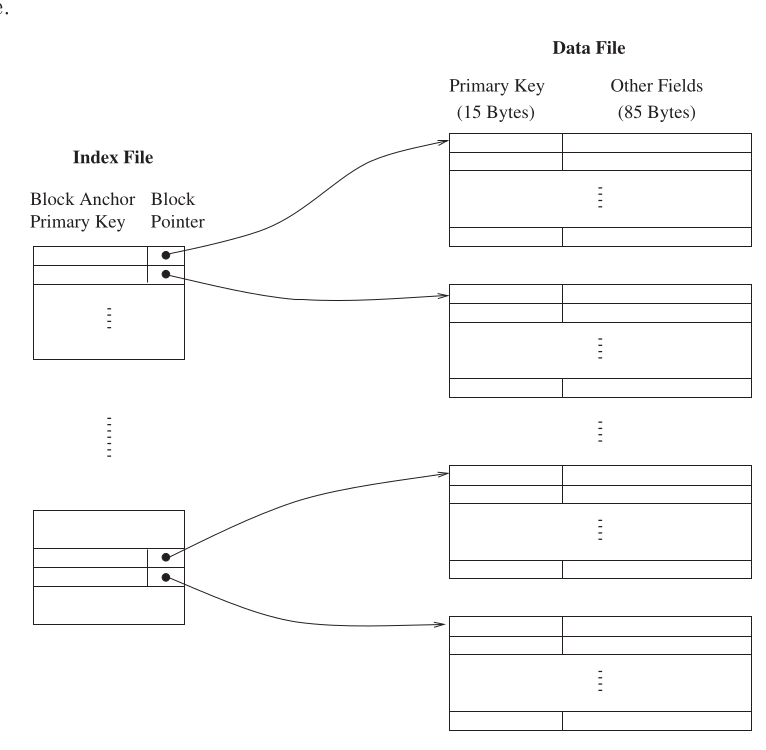
\includegraphics[width=0.7\linewidth]{figs/screenshot019}
				\caption{}
				\label{fig:screenshot019}
			\end{figure}
			
			
			Suppose the block size of the file system is $1024$ bytes, and a pointer to a block occupies $5$ bytes. The system uses binary search on the index file to search for a record with a given key. You may assume that a binary search on an index file of $b$ blocks takes [$\log_2 b$] block accesses in the worst case.
			
			Given a key, the number of block accesses required to identify the block in the data file that may contain a record with the key, in the worst case, is \underline{\hspace{2cm}}.
			
			\hfill $\brak{\text{GATE CS 2023}}$
			
			\item Consider the language $L$ over the alphabet $\{0, 1\}$, given below:
			
			$L = \{w \in \{0, 1\}^* \mid w \text{ does not contain three or more consecutive } 1\text{'s}\}$.
			
			The minimum number of states in a Deterministic Finite-State Automaton $\brak{\text{DFA}}$ for $L$ is \underline{\hspace{2cm}}.
			
			\hfill $\brak{\text{GATE CS 2023}}$
			
			\item An $8$-way set associative cache of size $64$ KB $\brak{1 \text{ KB} = 1024 \text{ bytes}}$ is used in a system with $32$-bit address. The address is sub-divided into TAG, INDEX, and BLOCK OFFSET.
			
			The number of bits in the TAG is \underline{\hspace{2cm}}.
			
			\hfill $\brak{\text{GATE CS 2023}}$
			
			\item The forwarding table of a router is shown below.
			
			\begin{table}[h]
				\centering
				\caption*{}
				\label{tab:forwarding}
				\begin{tabular}{|c|c|c|}
					\hline
					Subnet Number & Subnet Mask & Interface ID \\
					\hline
					$200.150.0.0$ & $255.255.0.0$ & $1$ \\
					\hline
					$200.150.64.0$ & $255.255.224.0$ & $2$ \\
					\hline
					$200.150.68.0$ & $255.255.255.0$ & $3$ \\
					\hline
					$200.150.68.64$ & $255.255.255.224$ & $4$ \\
					\hline
					Default & & $0$ \\
					\hline
				\end{tabular}
			\end{table}
			
			A packet addressed to a destination address $200.150.68.118$ arrives at the router. It will be forwarded to the interface with ID \underline{\hspace{2cm}}.
			
			\hfill $\brak{\text{GATE CS 2023}}$

		
	\end{enumerate}
\end{document}